\documentclass{article}
\usepackage[utf8]{inputenc}
\usepackage{amsmath}
\usepackage[dvipsnames]{xcolor}
\usepackage{pdfpages}
\usepackage{enumerate}
\usepackage{amssymb}
\usepackage[framemethod=default]{mdframed}
\usepackage[nomarginpar,left=2cm,right=2cm,top = 2cm, bottom = 2cm]{geometry}
\usepackage{standalone}
\usepackage{hyperref}
\usepackage{import}

\renewcommand{\thesubsection}{\thesection.\alph{subsection}}
\renewcommand{\thesubsubsection}{\thesection.\alph{subsection}.\roman{subsubsection}}

\mdfdefinestyle{theoremstyle}{%
linecolor=black,linewidth=.3pt,%
frametitlerule=true,%
frametitlebackgroundcolor=blue!5,
innertopmargin=\topskip,nobreak=true,
}

\mdfdefinestyle{style2}{frametitle={},%
             linewidth=.3pt,topline=true,backgroundcolor=blue!3!green!8!}

\mdtheorem[style=theoremstyle]{task}{Angabe}

\newmdenv[style = style2]{solution}

\mdfdefinestyle{style3}{frametitle={},%
             linewidth=.3pt,topline=true,backgroundcolor=red!15}

\newmdenv[style = style3]{disclaimer}

\begin{document}

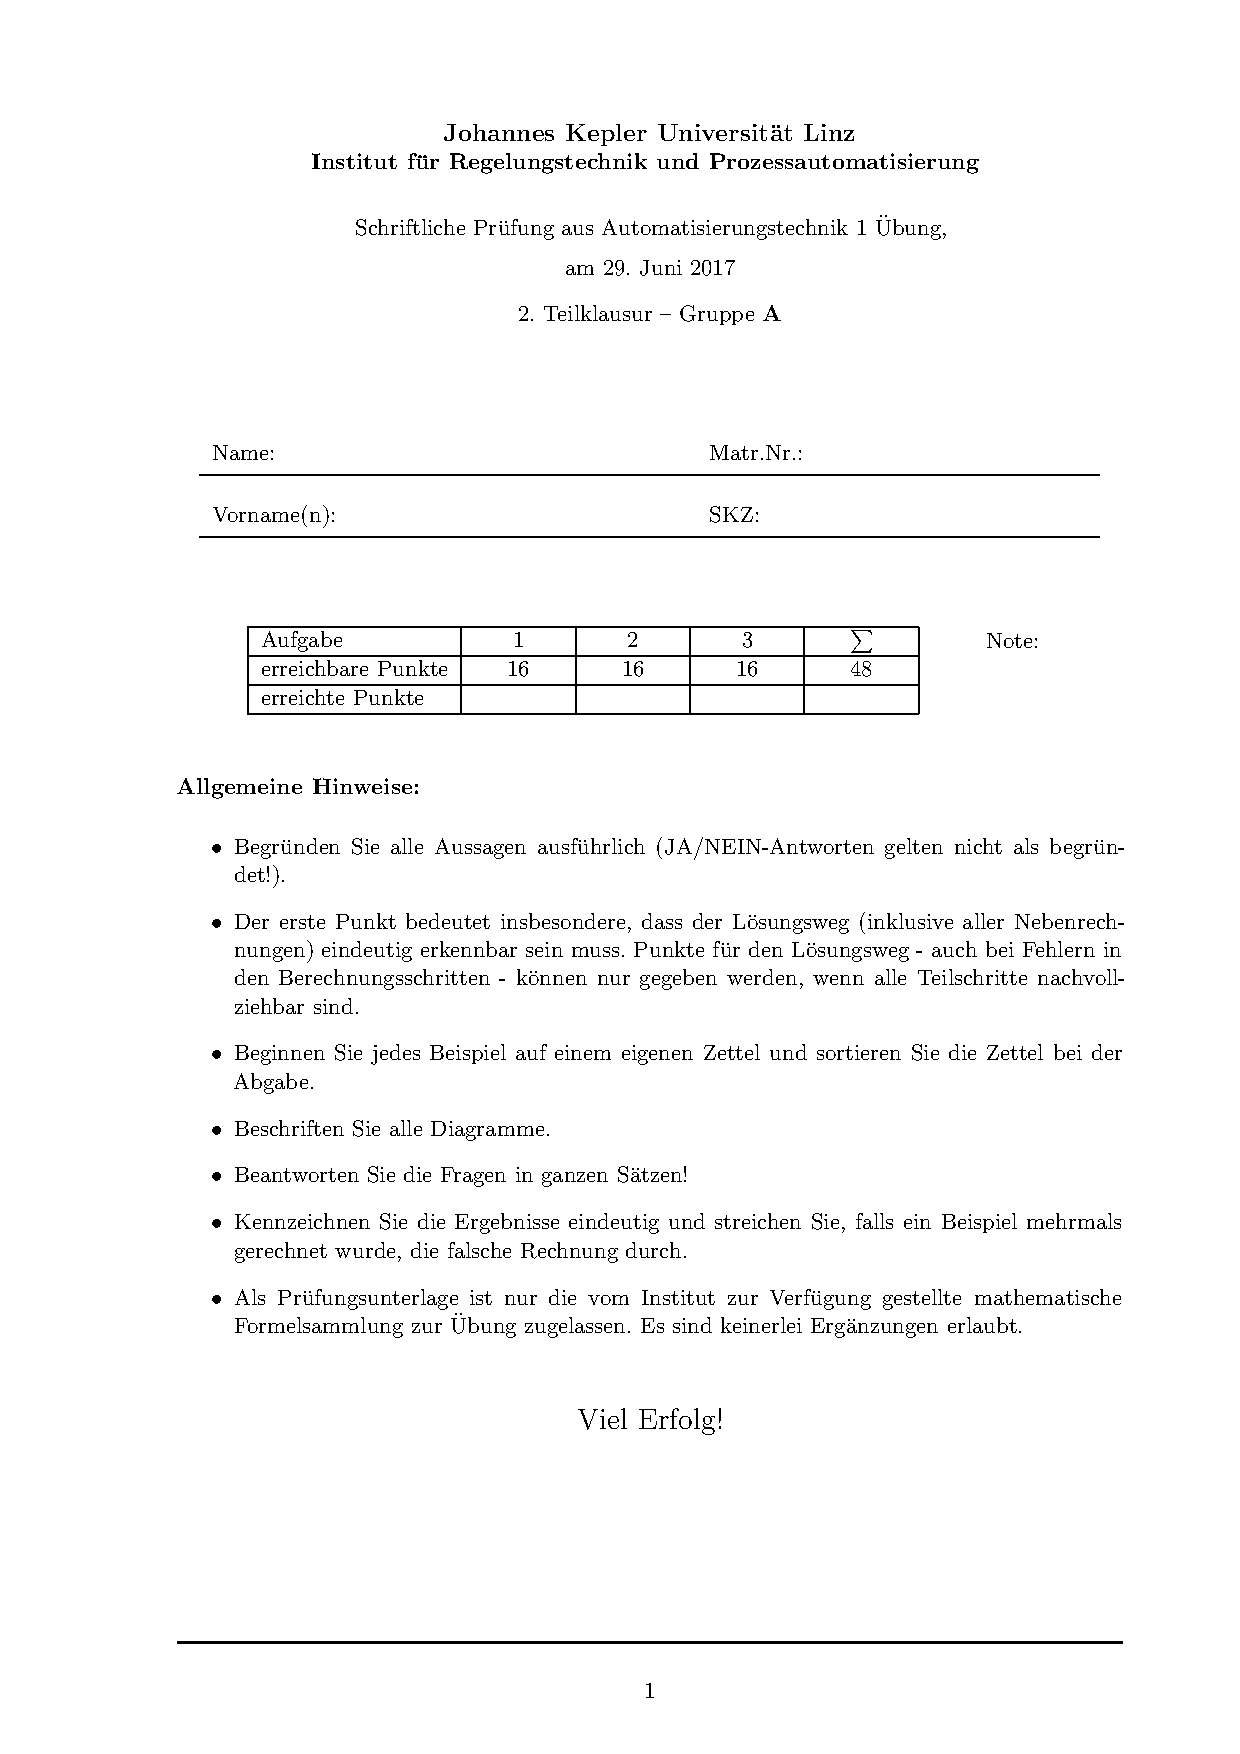
\includepdf[pages=-]{KlausurA_2017_06_29_nachtrKorrigiert}

\import{Subfiles/}{Disclaimer}
\import{Subfiles/}{Aufgabe1}
\import{Subfiles/}{Aufgabe2}
\import{Subfiles/}{Aufgabe3}
\import{Subfiles/}{Aufgabe4}
\import{Subfiles/}{Aufgabe5}
\import{Subfiles/}{Aufgabe6}


\end{document}
